\documentclass[10pt,twocolumn,a4paper]{article}

% =====================================================================
% Packages
% =====================================================================
\usepackage[utf8]{inputenc}
\usepackage[T1]{fontenc}
\usepackage[margin=2.1cm]{geometry}
\usepackage{amsmath,amssymb,amsthm,mathtools}
\usepackage{bm}
\usepackage{booktabs}
\usepackage{array}
\usepackage{graphicx}
\usepackage{caption}
\captionsetup{font=small,labelfont=bf}
\usepackage{enumitem}
\usepackage{lmodern}
\usepackage[expansion=false]{microtype}
\usepackage{algorithm}
\usepackage{algpseudocode}
\usepackage[hidelinks]{hyperref}
\usepackage[nameinlink,capitalise]{cleveref}
\crefname{assumption}{Assumption}{Assumptions}
\Crefname{assumption}{Assumption}{Assumptions}
\usepackage{natbib}
\bibliographystyle{unsrtnat}
\setcitestyle{numbers,square}

% =====================================================================
% Theorem environments
% =====================================================================
\newtheorem{theorem}{Theorem}[section]
\newtheorem{proposition}{Proposition}[section]
\newtheorem{lemma}{Lemma}[section]
\newtheorem{corollary}{Corollary}[section]
\theoremstyle{definition}
\newtheorem{definition}{Definition}[section]
\newtheorem{assumption}{Assumption}[section]
\theoremstyle{remark}
\newtheorem{remark}{Remark}[section]

% =====================================================================
% Notation
% =====================================================================
\newcommand{\MD}{{M_{\mathrm D}}}
\newcommand{\MN}{{M_{\mathrm N}}}
\newcommand{\WD}{W}
\newcommand{\WN}{{W_{\mathrm N}}}
\newcommand{\gainf}{g}
\newcommand{\incf}{\iota}
\newcommand{\resf}{\varrho}
\newcommand{\flam}{f_{\lambda}}
\newcommand{\lamhat}{\hat\lambda}
\newcommand{\CC}{\textsc{c}}
\newcommand{\DD}{\textsc{d}}
\newcommand{\UU}{\textsc{u}}
\newcommand{\Rset}{\mathbb{R}}
\newcommand{\E}{\mathbb{E}}
\newcommand{\Var}{\operatorname{Var}}
\newcommand{\se}{\mathrm{se}}

% =====================================================================
\title{\textbf{Rescue Is a Relation, Not a Trait: \\
Construction Dependence, Batch, and the Limits of Certification in a
Natural-Variation Screen for Rhizobacterial Drought Rescue in
\emph{Arabidopsis}}}

\author{%
Kundai Farai Sachikonye\\[0.2em]
\normalsize Experimental Bioinformatics, TUM School of Life Sciences\\
\normalsize Maximus-von-Imhof-Forum 3, 85354 Freising, Germany\\
\normalsize \texttt{kundai.sachikonye@bitspark.com}\\[0.6em]
\normalsize \textit{[Collaborator name and affiliation: data generation]}}

\date{\today}

% =====================================================================
\begin{document}
\maketitle

\begin{abstract}
\noindent
Natural-variation screens for plant responses to beneficial microbes
reduce a factorial experiment to a single number per accession and map
that number. In a screen of 247 \emph{Arabidopsis thaliana} accessions
inoculated with \emph{Pseudomonas simiae} WCS417 under drought, the
laboratory derived six families of such numbers (biomass under
inoculation, absolute gain, percentage increase, percentage rescue,
drought loss, and a binary rescuer label) and mapped each separately.
The candidate loci differed by trait, and no accession lost rescue. We
reanalyse the screen from its workbook alone. First, every derived trait
is an exact function of three cell means (inoculated--drought, mock--drought,
mock--non-stress), which we recover to $10^{-10}$ for all 235 complete
accessions; this exposes that one trait family uses no inoculated plants
at all and that the published ``tolerance'' table reports loss. Second,
we formalise a \emph{response construction} as a map from cell means to a
number that vanishes exactly when inoculation has no effect, and show
that the three constructions in use disagree about which accessions
rescue best: the top-20\% sets overlap by Jaccard 0.32--0.45 in shoot and
0.18--0.27 in root. Under a noise model that includes batch variation,
estimated from Col-0 grown in 13 blocks (intraclass correlation 0.28),
the shoot disagreement exceeds the resampling ceiling by at most 0.09
while the root disagreement exceeds it by 0.17--0.34, and under
plant-level noise alone the constructions
certify 63--700 pairs of accessions in \emph{opposite} order. Third, we
show that choosing a construction is equivalent to choosing an exponent
$\lambda$ in a scale-invariant family, that $\lambda$ is estimable from
the data, and that the data reject percentage increase ($\lambda=1$) in
both organs ($\lamhat=-0.26$ [$-0.57$, $-0.02$] shoot, $-0.04$ [$-0.26$,
$0.11$] root), after inverting a simulation-calibrated attenuation bias.
Within the data-admissible range, construction disagreement falls below
the noise ceiling. Fourth, comparing accessions through four columns (the
two mock baselines and the two inoculation responses) with a three-valued
verdict (correspond, diverge, decline) whose error rates we calibrate,
we find that the screen can certify divergence but essentially never
equivalence: the median pair becomes certifiable only at a margin of
1.7--2.8 between-accession standard deviations, and the screen resolves
four (shoot) to five (root) tiers of rescue. Of 28 candidate genes, none
recurs across trait families, three come from the mock-only trait, and
twelve come from a trait whose accession ranking correlates at 0.80 with
drought sensitivity. We give a replication design (independent runs
dominate plants per cell), a check that separates genuine rescue
enhancement from a weaker mock baseline, and a candidate loss-of-rescue
accession. The general conclusion is that ``rescue'' is a relation among
cells of a factorial, not a property of an accession, and that the
choice among its admissible readings must be made by the data, before
mapping, and reported.
\end{abstract}

\tableofcontents

% =====================================================================
\section{Introduction}
\label{sec:intro}
% =====================================================================

\subsection{The screen}

\emph{Pseudomonas simiae} WCS417 is a model plant-beneficial rhizobacterium
that promotes growth, reshapes root architecture and primes systemic
resistance in \emph{Arabidopsis} \citep{pieterse2014,zamioudis2013,berendsen2015}.
Part of its effect is linked to the plant's iron-deficiency machinery
\citep{zamioudis2015,stringlis2018,verbon2017}. A natural-variation screen
under non-stress conditions showed that nearly all accessions respond
positively, with large variation in the size of the response
\citep{wintermans2016}. Beneficial microbes are also candidates for
improving drought resilience \citep{devries2020}, which motivates the
screen we reanalyse here: 247 accessions grown with or without WCS417,
under non-stress or drought, with shoot and root fresh weight recorded,
followed by genome-wide association mapping \citep{atwell2010,grimm2017}.

The design has eight cells per accession (inoculation $\times$ water
regime $\times$ organ). Association mapping needs one number per
accession. The laboratory therefore derived several numbers and mapped
each of them:
\begin{itemize}[leftmargin=1.3em,itemsep=1pt]
  \item biomass under inoculation and drought;
  \item the absolute gain from inoculation under drought;
  \item the percentage increase from inoculation under drought;
  \item a percentage \emph{rescue} of the biomass lost to drought;
  \item the percentage biomass lost to drought;
  \item a binary rescuer label.
\end{itemize}
Different traits returned different candidate loci, and no accession was
found to lose rescue altogether. The absence of loss-of-rescue lines made
the usual contrast between responders and non-responders unavailable.

\subsection{The question}

Two questions follow and they are usually conflated. The first is
biological: which host loci modulate WCS417-mediated drought rescue? The
second is prior to it and methodological: \emph{which number is the
rescue of an accession?} A GWAS answers the first only after the second
has been answered, and the second is not answered by the data unless one
asks it explicitly. The candidate lists differ between traits. That
difference is either noise, which would argue for pooling, or it is
systematic, which would mean the traits measure different things and at
most one of them measures rescue.

Reducing a factorial to a ratio also has a long history of producing
artefacts. Ratios of noisy quantities correlate spuriously with their
own denominators \citep{pearson1897,kronmal1993}. Drought indices built
from stressed and unstressed yield are well known to conflate potential
with tolerance \citep{fischer1978,verslues2006}. Gene-by-environment
interaction is the rule in \emph{Arabidopsis}, not the exception
\citep{elsoda2014,desmarais2013}. None of this is new. What is missing is
a procedure that, given a screen like this one, says which readings of
the phenotype are admissible, lets the data choose among them, measures
how much the choice matters, and says how much any comparison between
accessions can be trusted.

\subsection{What this paper does}

We build that procedure from first principles and apply it to the
screen. \Cref{tab:contrib} lists the contributions.

\begin{table}[t]
\centering\small
\caption{Contributions, and where each is established.}
\label{tab:contrib}
\begin{tabular}{p{0.63\columnwidth}l}
\toprule
Contribution & Where \\
\midrule
Exact recovery of the unobserved cell means from derived traits; audit of labels & \S\ref{sec:audit} \\
Admissible response constructions; scale invariance; the $\lambda$ family & \S\ref{sec:constructions} \\
Heterogeneity and detectability of rescue & \S\ref{sec:res-het} \\
Construction dependence, measured against three noise models & \S\ref{sec:res-dep} \\
A data-driven choice of construction with bias correction & \S\ref{sec:res-can} \\
Four-column comparison with calibrated three-valued verdicts & \S\ref{sec:res-four} \\
Batch estimated from an internal control & \S\ref{sec:res-batch} \\
Consequences: candidate triage, mutant checks, design & \S\ref{sec:consequences} \\
\bottomrule
\end{tabular}
\end{table}

\subsection{What this paper does not do}
\label{sec:notdo}

\begin{enumerate}[label=(\arabic*),leftmargin=1.8em,itemsep=1pt]
  \item We do not rerun the association scan. The workbook contains no
  genotypes, and we did not retrieve them. Every statement about
  candidate loci concerns \emph{which trait} a candidate came from, not
  whether it is real.
  \item Per-plant values exist for one cell of the design only. For the
  other three cells we recover exact means but not their spread, so the
  noise in those cells is modelled, not measured
  (\Cref{ass:noise}). Every result that depends on this is reported under
  several noise models.
  \item We do not claim that any accession fails to be rescued. We
  identify accessions whose rescue is statistically compatible with zero;
  that is a reason to retest them, not a finding.
  \item We use no data beyond the workbook, the laboratory's slide deck,
  and the voice-recorded description of the design by the experimenter.
\end{enumerate}

% =====================================================================
\section{The screen as received}
\label{sec:data}
% =====================================================================

\paragraph{Materials.} The workbook contains six sheets:
\begin{itemize}[leftmargin=1.3em,itemsep=1pt]
  \item \emph{Biomass data}: per-plant rows;
  \item \emph{easyGWAS input}: one row per accession with 38 derived
  traits and two binary labels;
  \item \emph{easyGWAS output}: 40 candidate rows covering 28 genes;
  \item \emph{Accessions}: identifier, name, country and coordinates;
  \item \emph{Table 1} and \emph{Table 2}: summaries prepared for a
  manuscript.
\end{itemize}
Accessions are keyed by their 1001 Genomes identifiers \citep{genomes2016}.

\paragraph{What was measured and what was kept.}
The per-plant sheet holds 1,841 plants. \emph{All} of them belong to one
cell: WCS417-inoculated, drought. There are 243 accessions with 7 plants
each, three accessions (7394, 9807, 9874) with 14 plants in two blocks,
and Col-0 (6909) with 98 plants in 14 blocks, one of which has no
recorded weights. The mock plants and the non-stress plants appear only
through per-accession averages and medians embedded in the derived
traits. Primary root length is recorded for 1,042 plants.

\paragraph{Analysis set.} We exclude the four repeatedly grown lines,
because their derived traits were computed from inconsistent plant
subsets (\S\ref{sec:audit}). We also exclude eight accessions with
missing mock values. The analysis set is 235 accessions. Throughout,
``shoot'' and ``root'' refer to fresh weight in mg.

\paragraph{Collection sites.} The 235 accessions come from 30 countries,
led by Spain (66), Germany (44), Russia (18) and France (17). They are
not a random draw from the species. They are the collection that was
available in the laboratory, which had originally been assembled for a
study of annual precipitation. We return to this in
\S\ref{sec:res-geo}.

% =====================================================================
\section{Theory}
\label{sec:theory}
% =====================================================================

\subsection{Cell means and response constructions}
\label{sec:constructions}

For an accession $a$ and an organ, write
\[
  \WD_a,\quad M_{\mathrm D,a},\quad M_{\mathrm N,a},\quad W_{\mathrm N,a}
\]
for the mean fresh weights under inoculation--drought, mock--drought,
mock--non-stress and inoculation--non-stress respectively. The question
``how much does WCS417 rescue $a$ under drought?'' is a question about a
\emph{relation} among these cells, and there is more than one way to turn
it into a number.

\begin{definition}[Response construction]
\label{def:construction}
A \emph{response construction} is a function
$f:(\WD,\MD,\MN)\mapsto\Rset$, defined for $\MN>\MD>0$ and $\WD>0$,
with two properties:
\begin{enumerate}[label=(\roman*),leftmargin=1.8em,itemsep=0pt]
  \item \emph{null calibration}: $f=0$ if and only if $\WD=\MD$;
  \item \emph{monotonicity}: $f$ is strictly increasing in $\WD$.
\end{enumerate}
It is \emph{scale invariant} if, in addition,
$f(s\WD,s\MD,s\MN)=f(\WD,\MD,\MN)$ for every $s>0$.
\end{definition}

Scale invariance encodes a specific biological requirement. Accessions
differ in overall vigour, and a vigorous accession has larger fresh
weights in every cell. If rescue is a property of the interaction and not
of vigour, multiplying all four cells of an accession by the same factor
should leave its rescue unchanged. The three constructions used in the
screen are:
\begin{align}
  \gainf &= \WD-\MD, \label{eq:gain}\\
  \incf  &= \WD/\MD-1, \label{eq:inc}\\
  \resf  &= (\WD-\MD)/(\MN-\MD). \label{eq:res}
\end{align}
Here $\gainf$ is the absolute gain, $\incf$ the proportional increase
over the mock plant under the same drought, and $\resf$ the fraction of
the drought loss that inoculation restores.

\begin{proposition}[Which constructions are scale invariant]
\label{prop:scale}
All three constructions are admissible. Of them, $\incf$ and $\resf$ are
scale invariant and $\gainf$ is not.
\end{proposition}
\begin{proof}
Null calibration and monotonicity are immediate in each case, because
$\MD>0$ and $\MN-\MD>0$. Under $(\WD,\MD,\MN)\mapsto s(\WD,\MD,\MN)$,
$\gainf\mapsto s\gainf$, whereas the numerator and the denominator of
$\incf+1$ and of $\resf$ both scale by $s$.
\end{proof}

The two scale-invariant constructions are members of one family.

\begin{definition}[The $\lambda$ family]
\label{def:lambda}
For $\lambda\in\Rset$ let
\begin{equation}
  \flam(\WD,\MD,\MN)=\frac{\WD-\MD}{\MD^{\lambda}\,(\MN-\MD)^{1-\lambda}}.
  \label{eq:flam}
\end{equation}
Then $f_1=\incf$ and $f_0=\resf$.
\end{definition}

The denominator is homogeneous of degree one, so every $\flam$ is scale
invariant. The exponent $\lambda$ says which baseline the gain is
measured against: the size of the stressed mock plant ($\lambda=1$), the
size of the drought loss ($\lambda=0$), or a geometric compromise. The
following proposition makes precise the sense in which choosing $\lambda$
\emph{is} choosing a mechanism.

\begin{proposition}[The construction encodes a null mechanism]
\label{prop:mechanism}
Suppose the gains are generated as
\begin{equation}
  \WD_a-M_{\mathrm D,a}=\theta_a\,M_{\mathrm D,a}^{\lambda^*}\,(M_{\mathrm N,a}-M_{\mathrm D,a})^{1-\lambda^*},
  \label{eq:gen}
\end{equation}
with a rescue capacity $\theta_a>0$ that is statistically independent of
the baselines $(M_{\mathrm D,a},M_{\mathrm N,a})$. Then:
\begin{enumerate}[label=(\roman*),leftmargin=1.8em,itemsep=0pt]
  \item $f_{\lambda^*}(a)=\theta_a$ is independent of both baselines;
  \item for any $\lambda\neq\lambda^*$,
  \[
    \flam(a)=\theta_a\bigl(M_{\mathrm D,a}/(M_{\mathrm N,a}-M_{\mathrm D,a})\bigr)^{\lambda^*-\lambda},
  \]
  which depends on the baselines unless $\MD/(\MN-\MD)$ is constant
  across accessions.
\end{enumerate}
\end{proposition}
\begin{proof}
Substitute \eqref{eq:gen} into \eqref{eq:flam}.
\end{proof}

The ratio $\MD/(\MN-\MD)$ is a monotone transform of drought
sensitivity: it is small when drought removes most of the biomass. So the
wrong $\lambda$ loads the phenotype onto drought sensitivity, and the
sign of $\lambda^*-\lambda$ sets the direction of the loading.
Percentage increase is the right construction only if WCS417 multiplies
the stressed biomass by an accession-specific factor. Rescue is the right
one only if WCS417 restores an accession-specific fraction of the
biomass lost. Nothing in the definition of ``rescue'' decides between
these; the data can.

\paragraph{Estimating $\lambda$.} Taking logarithms of \eqref{eq:gen}
gives a linear model
\begin{equation}
  \log(\WD-\MD)=b_0+b_1\log\MD+b_2\log(\MN-\MD)+\varepsilon,
  \label{eq:loglin}
\end{equation}
in which the mechanism predicts $b_1=\lambda^*$ and $b_1+b_2=1$. The
second of these is scale invariance of the mechanism itself, and is
testable. Because $\MD$ enters both sides with measurement error, the
ordinary least-squares $b_1$ is biased \citep{carroll2006}. We estimate
the bias by simulation at the observed noise level and invert it
(\S\ref{sec:methods-lambda}).

\subsection{Receiver relativity}
\label{sec:relativity}

Let $y_a=f(a)$ be the response of accession $a$ under a fixed
construction, and $\se_a$ its standard error. If WCS417 had one effect
on all accessions, the $y_a$ would differ only by noise.

\begin{definition}[Heterogeneity]
\label{def:het}
With inverse-variance weights $w_a=\se_a^{-2}$ and weighted mean $\bar y$,
Cochran's statistic \citep{cochran1954}
\[
  Q=\sum_a w_a(y_a-\bar y)^2
\]
is $\chi^2_{n-1}$ under a common effect. The excess
$I^2=(Q-(n-1))/Q$ \citep{higgins2002} and the reliability
\[
  \mathcal R=\frac{\tau^2}{\tau^2+\overline{\se^2}},\qquad
  \tau^2=\Var(y)-\overline{\se^2},
\]
measure how much of the observed spread is between accessions.
\end{definition}

$\mathcal R$ plays the role of an entry-mean repeatability
\citep{falconer1996,lynch1998}: it bounds the variance that any locus
could explain. A large $Q$ means the effect of the strain has no single
value. It has one value per accession, each a property of the pair
(strain, accession), and the object of a mapping study is that indexed
set, not a number attached to the strain.

\subsection{Construction independence}
\label{sec:independence}

Let $\mathcal F$ be a set of admissible constructions and let $V_f$ be a
verdict computed from construction $f$. Examples of verdicts are the set
of the top $k$ accessions, or the certified order of a pair.

\begin{definition}[Construction independence]
\label{def:ci}
A verdict is \emph{construction independent over $\mathcal F$ at noise
level $\mathcal M$} if, for all $f,g\in\mathcal F$, the disagreement
between $V_f$ and $V_g$ on the observed data does not exceed the
disagreement between $V_f$ on the observed data and $V_f$ on data
resampled under the noise model $\mathcal M$ (95th percentile).
\end{definition}

The comparison is the substance of the definition. Two constructions can
disagree because they read the same truth differently, or because each
is noisy. Only the first is a property of the constructions, and it is
detectable only as disagreement beyond what resampling produces.

A stronger failure than disagreement is contradiction.

\begin{definition}[Certified order; decisive contradiction]
\label{def:order}
Construction $f$ \emph{certifies} $a\succ b$ if
\[
  f(a)-f(b)-z_\alpha\sqrt{\se_a^2+\se_b^2}>\delta.
\]
Two constructions are in \emph{decisive contradiction} on a pair if one
certifies $a\succ b$ and the other certifies $b\succ a$.
\end{definition}

\subsection{Four columns and three-valued verdicts}
\label{sec:fourcol}

Comparing two accessions by their response alone discards what they
share. Two accessions can have the same response for different reasons,
or different responses from indistinguishable starting points. We
therefore compare a pair $(a,b)$ through four columns:
\begin{itemize}[leftmargin=1.3em,itemsep=1pt]
  \item two \emph{baseline} columns, the mock phenotype vector
  $(\log\MD,\log\MN)$ of $a$ and of $b$;
  \item two \emph{response} columns, $f(a)$ and $f(b)$.
\end{itemize}
Each pair of columns is compared by a verdict with three values.

\begin{definition}[Three-valued verdict]
\label{def:verdict}
For an observed difference $d$ with standard error $s$ and a margin
$\delta>0$, set
\[
  V(d,s;\delta)=
  \begin{cases}
  \CC\ (\text{correspond}) & |d|+z_\alpha s<\delta,\\
  \DD\ (\text{diverge})    & |d|-z_\alpha s>\delta,\\
  \UU\ (\text{decline})    & \text{otherwise},
  \end{cases}
\]
with $z_\alpha$ the one-sided $1-\alpha$ normal quantile.
\end{definition}

For a two-component baseline, the verdict is \CC\ if both components are
\CC, \DD\ if either is \DD, and \UU\ otherwise (intersection--union).

\CC\ is the two one-sided tests rule for equivalence
\citep{schuirmann1987,lehmann2005}. \DD\ is its mirror image:
a certification that the difference exceeds the margin. \UU\ is not a
failure of the procedure. It is the correct report when the data do not
settle the question, and a procedure without it must return a confident
answer for every pair.

\begin{proposition}[Error control]
\label{prop:error}
Let $d\sim\mathcal N(\Delta,s^2)$ with $s$ known. Then
\begin{enumerate}[label=(\roman*),leftmargin=1.8em,itemsep=0pt]
  \item $\Pr[V=\CC]\le\alpha$ whenever $|\Delta|\ge\delta$;
  \item $\Pr[V=\DD]\le\alpha+\Phi(-2\delta/s-z_\alpha)$ whenever
  $|\Delta|\le\delta$.
\end{enumerate}
\end{proposition}
\begin{proof}
(i) Take $\Delta\ge\delta$ without loss of generality. \CC\ requires
$d<\delta-z_\alpha s$, which has probability
$\Phi((\delta-\Delta)/s-z_\alpha)\le\Phi(-z_\alpha)=\alpha$.

(ii) \DD\ requires $d>\delta+z_\alpha s$ or $d<-\delta-z_\alpha s$. For
$|\Delta|\le\delta$, the first has probability at most $\alpha$, attained
at $\Delta=\delta$. The second is then
$\Phi(-2\delta/s-z_\alpha)$ at the same $\Delta$, and smaller elsewhere.
\end{proof}

The four columns define a $3\times 3$ table of (baseline, response)
verdicts. Two cells of it carry the diagnostic content:
\begin{itemize}[leftmargin=1.3em,itemsep=1pt]
  \item (\CC, \DD): \emph{false friends}, indistinguishable in mock but
  different in response;
  \item (\DD, \CC): \emph{convergent} pairs, different in mock but
  equivalent in response.
\end{itemize}
A comparison that reads only the response columns cannot tell a false
friend from an ordinary divergent pair. A comparison that reads only the
biomass under inoculation mixes the columns altogether.

\begin{definition}[Minimum certifiable margin]
\label{def:dmin}
For a pair, $\delta_{\min}=|d|+z_\alpha s$. This is the smallest margin at
which the pair would be certified \CC.
\end{definition}

The distribution of $\delta_{\min}$ over pairs, expressed in units of the
between-accession standard deviation, is a design-level quantity. It says
how coarse a notion of ``the same rescue'' the screen can support at
all. If the median pair needs a margin larger than the population spread,
the screen cannot certify any meaningful equivalence.

\begin{definition}[Resolution depth]
\label{def:depth}
Let $a\succ b$ mean certified order at margin $0$. The \emph{resolution
depth} is the length of the longest chain $a_1\succ a_2\succ\cdots\succ
a_L$. The \emph{tier} of an accession is the length of the longest chain
ending at it from below.
\end{definition}

Resolution depth counts how many levels of rescue the screen can tell
apart, which matters more to a follow-up experiment than how many
accessions it ranks.

\subsection{Noise models}
\label{sec:noise}

\begin{assumption}[Noise]
\label{ass:noise}
Cell means are perturbed multiplicatively and log-normally. The plant
coefficient of variation $c_p$ is the median within-accession coefficient
of variation of the observed inoculated--drought plants, and it is
assumed to hold in the three unobserved cells. The batch coefficient of
variation $c_b$ is the between-block excess variance of Col-0 block
means (\S\ref{sec:res-batch}). Batch effects are independent across
cells.
\end{assumption}

The last clause is conservative. If an accession's mock and inoculated
plants shared a tray, part of the batch effect would cancel in $\WD-\MD$.
We therefore bracket the truth with four models:
\begin{description}[leftmargin=1.3em,itemsep=1pt,font=\normalfont\itshape]
  \item[M1] resample the observed inoculated plants; mock means fixed.
  \item[M2] M1, plus mock means perturbed with coefficient of variation
  $c_p/\sqrt 7$.
  \item[M3] M2, plus a batch factor on every cell. This is the reference
  model.
  \item[M4] M3 with the mock noise multiplied by 1.5.
\end{description}
We read M2 and M3 as lower and upper bounds on realistic noise.

\subsection{Estimating $\lambda$ without bias}
\label{sec:methods-lambda}

\paragraph{Uncertainty.} We fit \eqref{eq:loglin} by ordinary least
squares and bootstrap \citep{efron1979} jointly over accessions (case
resampling) and noise (a fresh M3 draw per replicate), with 1,000
replicates.

\paragraph{Bias.} To calibrate, we simulate synthetic screens for
$\lambda^*\in\{-0.75,-0.5,\dots,1\}$:
\begin{itemize}[leftmargin=1.3em,itemsep=1pt]
  \item the observed $(\MD,\MN)$ are taken as the true baselines;
  \item $\log\theta_a$ is normal with the residual standard deviation of
  the observed fit;
  \item gains are scaled to the observed median, and M3 noise is added.
\end{itemize}
We run 200 replicates per value of $\lambda^*$. The mean estimate is
monotone in $\lambda^*$. We invert that curve to obtain a corrected
$\lamhat$, and apply the same inversion to the bootstrap interval.

% =====================================================================
\section{Results}
\label{sec:results}
% =====================================================================

\begin{figure*}[!htbp]
  \centering
  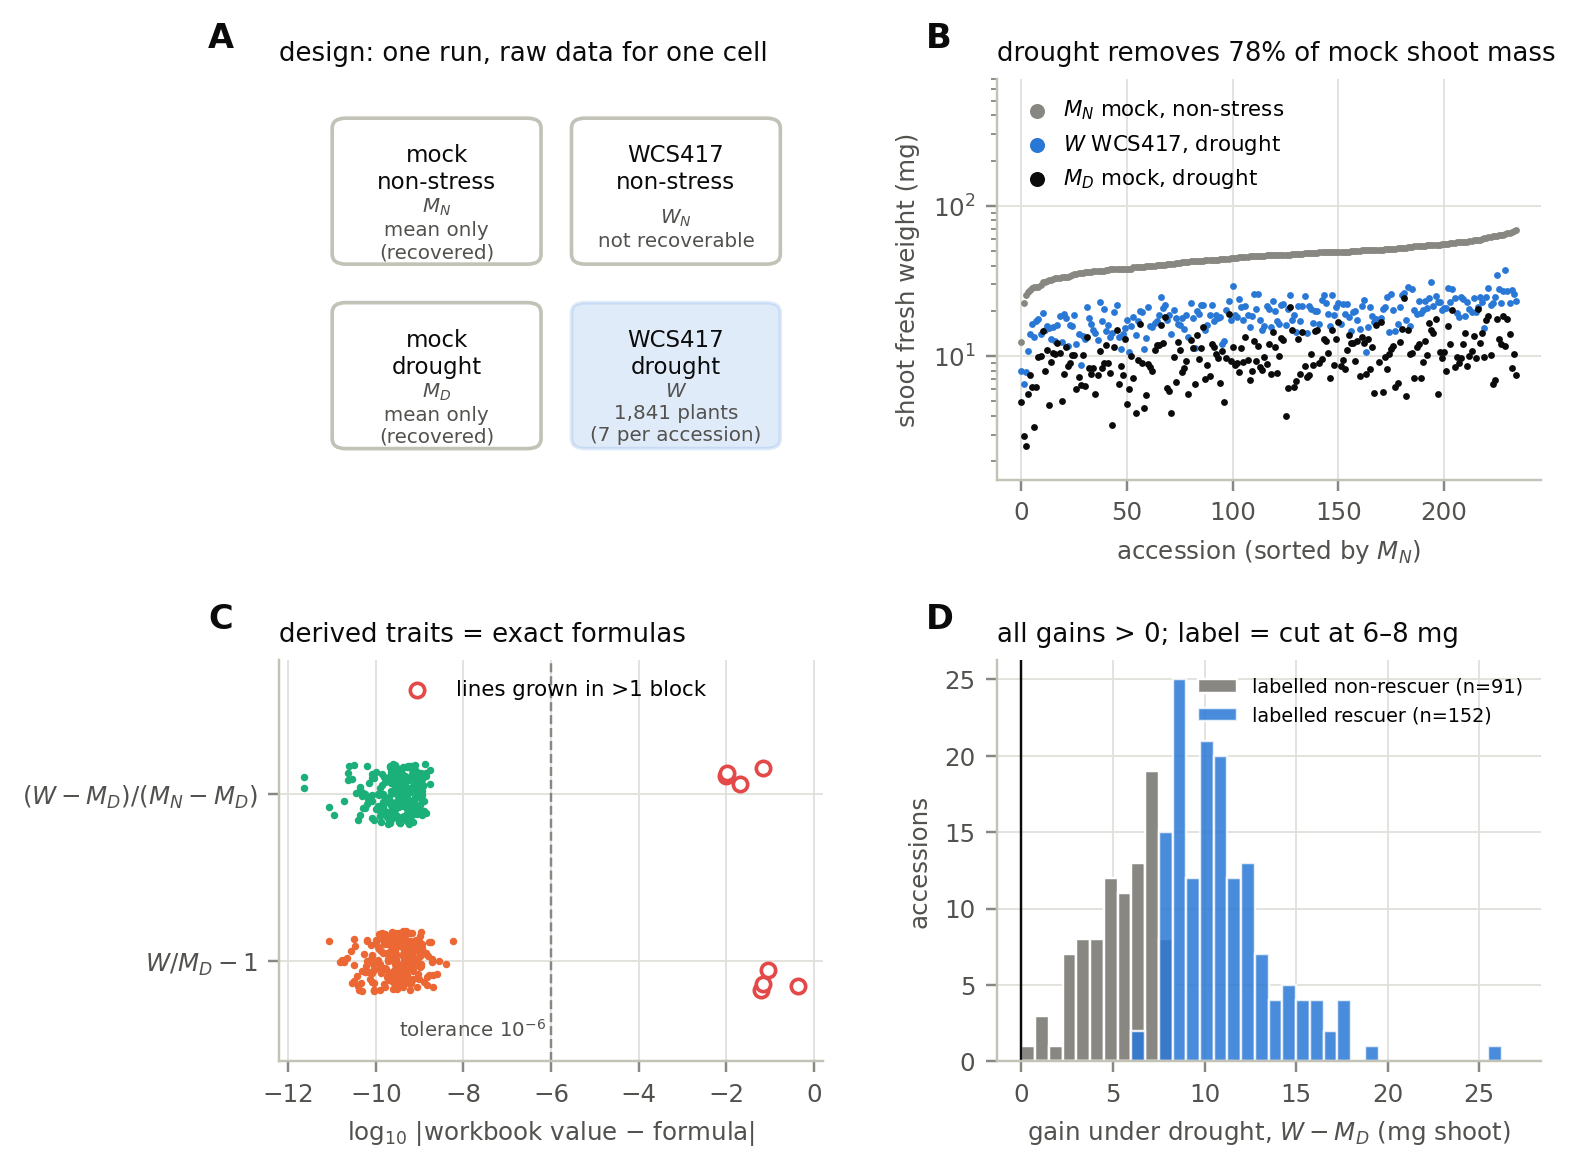
\includegraphics[width=\textwidth]{figures/panel_1_audit.png}
  \caption{\textbf{The workbook determines three of four cell means exactly, and one trait family uses no inoculated plants.}
  (\textbf{A})~Design and data availability. Per-plant weights exist only for WCS417--drought (1,841 plants). Mock means are recovered from the derived traits (\S\ref{sec:audit}). WCS417--non-stress cannot be recovered, because the one trait that involves it admits two readings.
  (\textbf{B})~Recovered shoot cell means for 235 accessions, sorted by $\MN$, on a log scale. Drought removes a median 78\% of mock shoot biomass (84\% of root). Inoculation recovers a varying part of it.
  (\textbf{C})~Absolute residual between each workbook trait and its closed form, on a log scale. For all 235 accessions in the analysis set, the rescue and increase traits equal \eqref{eq:res} and \eqref{eq:inc} to rounding error (median $4\times10^{-10}$). The four exceptions (red) are the lines grown in more than one block, whose traits mix plant subsets.
  (\textbf{D})~Distribution of the shoot gain $\WD-\MD$ by the workbook's binary label. No accession has a negative gain: the smallest is 0.73~mg. The label is a cut between 6.1 and 7.8~mg, not a loss of rescue.}
  \label{fig:audit}
\end{figure*}

\subsection{Audit of the workbook}
\label{sec:audit}

\paragraph{Recovering the cell means (\Cref{fig:audit}).} The absolute
gain under drought and the percentage loss under drought determine the
mock means exactly:
\[
  \MD=\WD-\text{gain}_{\mathrm D},\qquad \MN=\MD/(1-\text{loss}).
\]
Because $\WD$ is the mean of the recorded plants (maximum discrepancy
$4\times10^{-9}$), both mock cells follow for every accession.

\paragraph{Checking the recovery.} Two traits not used in the recovery
serve as independent checks:
\begin{itemize}[leftmargin=1.3em,itemsep=1pt]
  \item the workbook's percentage rescue equals \eqref{eq:res} for all
  235 accessions (median absolute residual $3.8\times10^{-10}$ shoot,
  $5.9\times10^{-10}$ root);
  \item the percentage increase equals \eqref{eq:inc} for 239 of 247.
\end{itemize}
The only failures of either identity are the four repeatedly grown lines,
with residuals 0.007--0.13. Their traits were computed from differing
plant subsets, and we exclude them.

\paragraph{The unrecoverable cell.} The ``gain under non-stress'' trait
is consistent to rounding error with two different definitions,
$\WN-\MN$ and $\WD-\WN$. $\WN$ is therefore not identifiable from the
workbook, and no analysis below uses it.

\paragraph{Three corrections to the laboratory's reading.}
\begin{enumerate}[label=(\roman*),leftmargin=1.8em,itemsep=1pt]
  \item The ``loss under drought'' trait, $1-\MD/\MN$, uses mock plants
  only. It measures drought sensitivity, not rescue.
  \item The ``drought tolerance'' columns of the laboratory's Table~2 are
  identical to that loss for 239 of 240 accessions. A larger value
  therefore means \emph{less} tolerance, the opposite of what the label
  says.
  \item The binary rescuer label is a threshold on a positive gain
  (\Cref{fig:audit}D). Labelled non-rescuers gain 0.73--7.75~mg shoot;
  labelled rescuers gain 6.09--25.6~mg. Every accession gains.
\end{enumerate}
Table~1 of the laboratory reports the drought condition: its mock and
WCS417 columns match $\MD$ and $\WD$ with $r=0.96$ and $0.97$
($n=243$).

\begin{figure*}[!htbp]
  \centering
  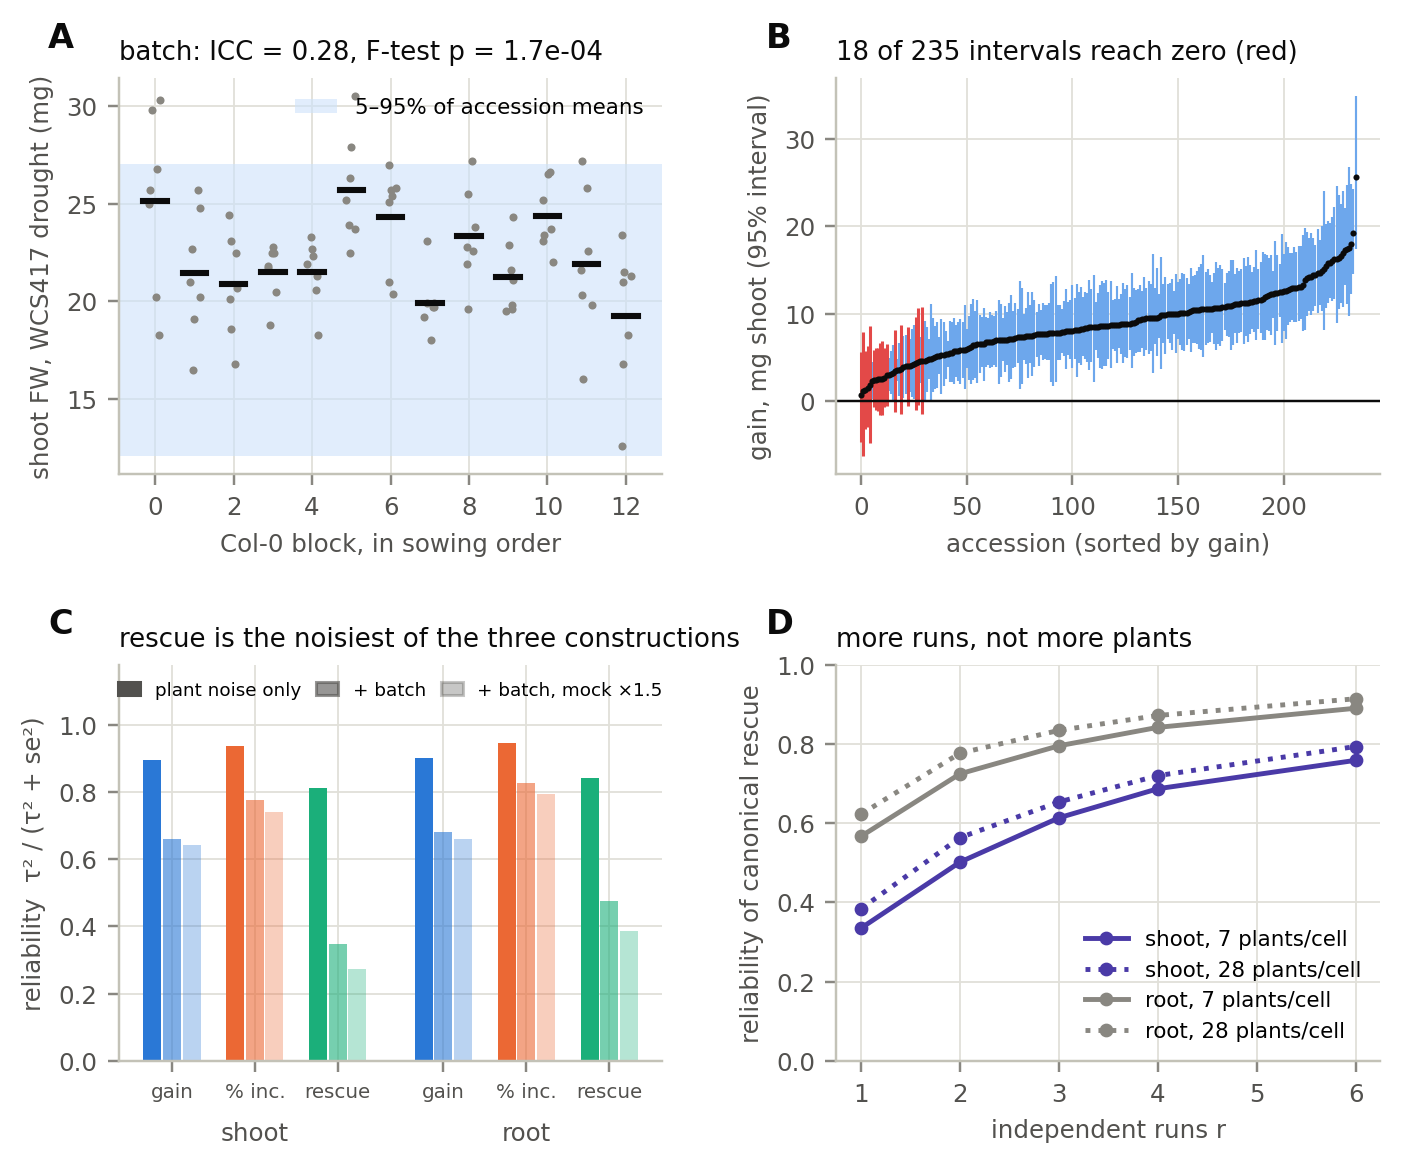
\includegraphics[width=\textwidth]{figures/panel_2_noise.png}
  \caption{\textbf{Batch is a first-order component of noise, rescue is the least reliable construction, and replication should add runs.}
  (\textbf{A})~Col-0 was grown in 13 usable blocks of 7 plants spread through the screen. Block means (bars) differ beyond plant noise ($F=3.76$, $p=1.7\times10^{-4}$, ICC $=0.28$). The spread of the block means is 0.43 of the between-accession spread, and Col-0 alone moves from the 54th to the 92nd percentile of accessions.
  (\textbf{B})~Shoot gain with 95\% intervals under the reference noise model (M3), sorted. Eighteen of 235 intervals include zero (red). Under plant noise alone (M2) six do. Per-1 is compatible with zero in shoot and root under every model.
  (\textbf{C})~Reliability $\mathcal R$ (\Cref{def:het}) by construction and noise model. Adding batch noise lowers the reliability of rescue to 0.35 (shoot) and 0.48 (root); the other two constructions remain between 0.66 and 0.83. Heterogeneity is significant for every construction, organ and model (\Cref{tab:het}).
  (\textbf{D})~Reliability of the canonical construction as a function of independent runs $r$, for 7 and 28 plants per cell. Quadrupling the plants moves reliability by at most 0.05; a second run moves it by 0.15--0.17.}
  \label{fig:noise}
\end{figure*}

\subsection{Heterogeneity and detectability}
\label{sec:res-het}

\paragraph{Noise parameters.} The plant coefficient of variation is
$c_p=0.121$ (shoot) and $0.156$ (root). Col-0 gives $c_b=0.081$ and
$0.093$.

\paragraph{Heterogeneity.} Inoculation effects differ between accessions
far beyond noise, for every construction, organ and noise model
(\Cref{tab:het}). Under M3 the shoot $Q$ ranges from 396 to 877 on 234
degrees of freedom. So the effect of WCS417 under drought is
receiver-relative in the sense of \S\ref{sec:relativity}: it has no
single value.

\begin{table}[t]
\centering\small
\caption{Heterogeneity of the inoculation effect across 235 accessions
(df $=234$). $\mathcal R$ is the reliability. All $p<10^{-9}$.}
\label{tab:het}
\begin{tabular}{llrrr}
\toprule
Organ & Construction & $Q$ (M2) & $Q$ (M3) & $\mathcal R$ (M3) \\
\midrule
Shoot & gain     & 3,422 & 757 & 0.66 \\
      & increase & 3,692 & 877 & 0.78 \\
      & rescue   & 1,710 & 396 & 0.35 \\
Root  & gain     & 3,869 & 931 & 0.68 \\
      & increase & 3,879 & 1,048 & 0.83 \\
      & rescue   & 1,899 & 516 & 0.48 \\
\bottomrule
\end{tabular}
\end{table}

\paragraph{Reliability.} Reliability differs sharply between
constructions. Rescue, a ratio of two differences, is the noisiest. Under
M3 its between-accession standard deviation is smaller than its
per-accession standard error (ratio 0.77 in shoot). A GWAS on shoot rescue
from this screen maps a phenotype of which about a third of the variance
is between accessions.

\paragraph{Could a loss of rescue have been detected?} Under M3 the
median shoot gain is 4.5 standard errors from zero, and 92\% of
accessions have intervals that exclude zero (96\% in root). The minimum
gain detectable with 80\% power is 5.8~mg shoot, against an observed
median of about 9~mg. A complete loss of rescue in most genetic
backgrounds would therefore have been visible.

\paragraph{Retest candidates.} Eighteen shoot intervals and nine root
intervals include zero under M3. Under M2 the numbers are six (shoot) and
one (root). Per-1 has the smallest gain in both organs (0.73~mg shoot,
0.27~mg root) and is compatible with zero under every model. It is the
natural first candidate for retesting as a loss-of-rescue line.

\begin{figure*}[!htbp]
  \centering
  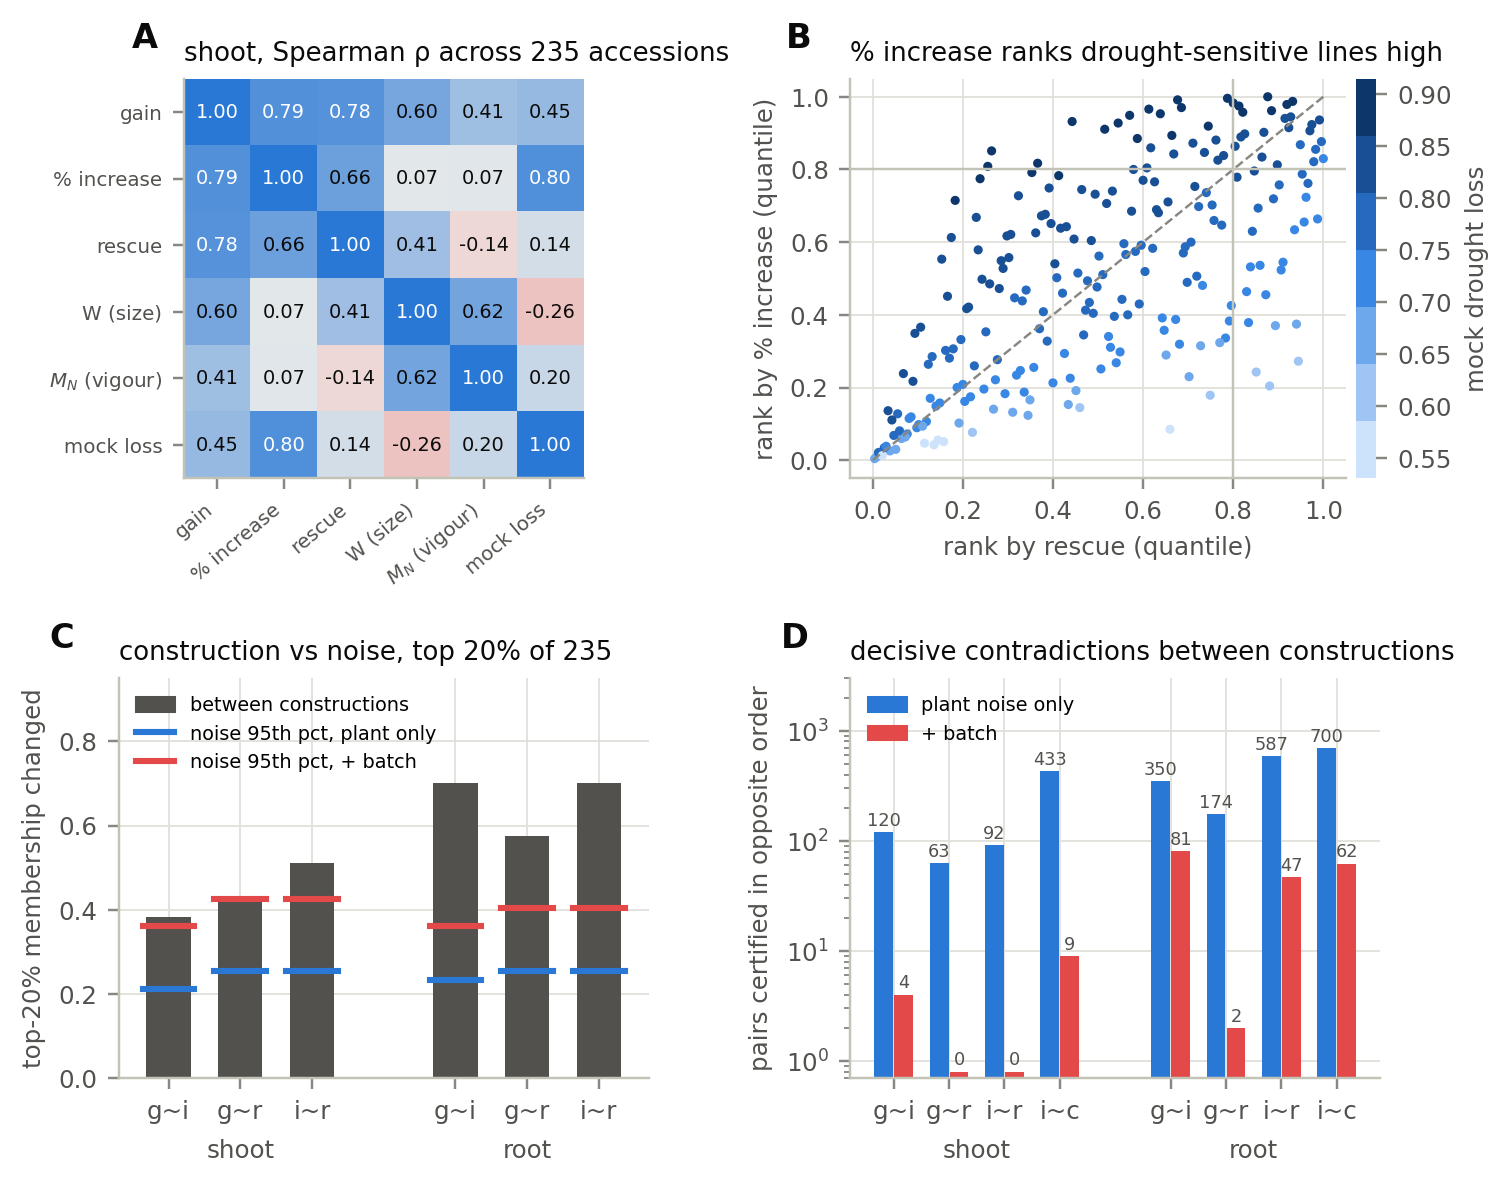
\includegraphics[width=\textwidth]{figures/panel_3_dependence.png}
  \caption{\textbf{The three constructions in use disagree about which accessions rescue best, and sometimes certify opposite orders.}
  (\textbf{A})~Spearman correlations across 235 accessions (shoot) between the constructions and three nuisance quantities: size under inoculation $\WD$, vigour $\MN$, and mock-only drought loss. Percentage increase is nearly uncorrelated with size but correlates at 0.80 with drought loss. Gain correlates at 0.60 with size. Rescue is the least loaded on either.
  (\textbf{B})~Rank by percentage increase against rank by rescue, coloured by drought loss. Accessions far above the diagonal are drought-sensitive: their small $\MD$ inflates the ratio.
  (\textbf{C})~Fraction of the top 20\% (47 accessions) that changes between two constructions (bars), against the 95th percentile of the same fraction under resampling of one construction: plant noise (blue) and plant + batch noise (red). In root every pair exceeds even the batch-inclusive ceiling (0.57--0.70 against 0.36--0.40).
  (\textbf{D})~Pairs of accessions certified in \emph{opposite} order by two constructions (\Cref{def:order}, $\delta=0.5$ SD). Under plant noise these number 63--433 in shoot and 174--700 in root. With batch noise they fall to 0--81.}
  \label{fig:dep}
\end{figure*}

\subsection{Construction dependence}
\label{sec:res-dep}

\paragraph{Correlations (\Cref{fig:dep}A).} The three constructions are
correlated but far from interchangeable. The pairwise Spearman
correlations \citep{spearman1904} are:
\begin{itemize}[leftmargin=1.3em,itemsep=1pt]
  \item gain with increase 0.79 and gain with rescue 0.78, but increase
  with rescue only 0.66 (shoot);
  \item 0.59, 0.61 and 0.41 respectively in root.
\end{itemize}

\paragraph{Why they disagree (\Cref{fig:dep}A, B).} Each construction
carries a different nuisance, as \Cref{prop:mechanism} predicts.
\begin{itemize}[leftmargin=1.3em,itemsep=1pt]
  \item Percentage increase ranks accessions almost as mock-only drought
  loss does ($\rho=0.80$ in both organs). A drought-sensitive accession
  has a small $\MD$ and hence a large ratio. This is the spurious ratio
  correlation of \citet{pearson1897}, reappearing as a phenotype.
  \item Gain in milligrams tracks size ($\rho=0.60$ with $\WD$).
  \item Rescue is loaded on neither beyond $|\rho|=0.41$, but it is the
  least reliable (\Cref{tab:het}).
\end{itemize}

\paragraph{Top sets (\Cref{fig:dep}C).} The top-20\% sets overlap by
Jaccard index \citep{jaccard1912} 0.32--0.45 in shoot and 0.18--0.27 in
root. Only 15 of 47 shoot accessions, and 7 of 47 root accessions, are in
the top fifth under all three constructions. At the top 10\% no root
accession is shared by all three.

Against the noise ceilings of \Cref{def:ci}:
\begin{itemize}[leftmargin=1.3em,itemsep=1pt]
  \item \emph{Shoot.} Construction disagreement exceeds the plant-noise
  ceiling for every pair (e.g.\ 0.51 against 0.26 for increase--rescue)
  but exceeds the batch-inclusive ceiling only marginally (0.51 against
  0.43; excess 0.00--0.09 across the three pairs).
  \item \emph{Root.} It exceeds both ceilings for every pair, by
  0.17--0.34.
\end{itemize}
So construction independence fails in root under every noise model. In
shoot it fails clearly without batch noise. With batch noise the
construction question is nearly swamped, but only because the screen
itself becomes too noisy to rank.

\paragraph{Contradictions (\Cref{fig:dep}D).} Disagreement is not only a
matter of which verdicts are reached; some verdicts are reversed. Under
plant noise, percentage increase and the canonical construction
(\S\ref{sec:res-can}) certify 433 shoot pairs and 700 root pairs in
opposite order. Under the batch-inclusive model 9 and 62 such
contradictions survive. A contradiction is not a disagreement about
resolution. It is two admissible readings of the same data asserting,
each at the 5\% level, incompatible facts.

\begin{figure*}[!htbp]
  \centering
  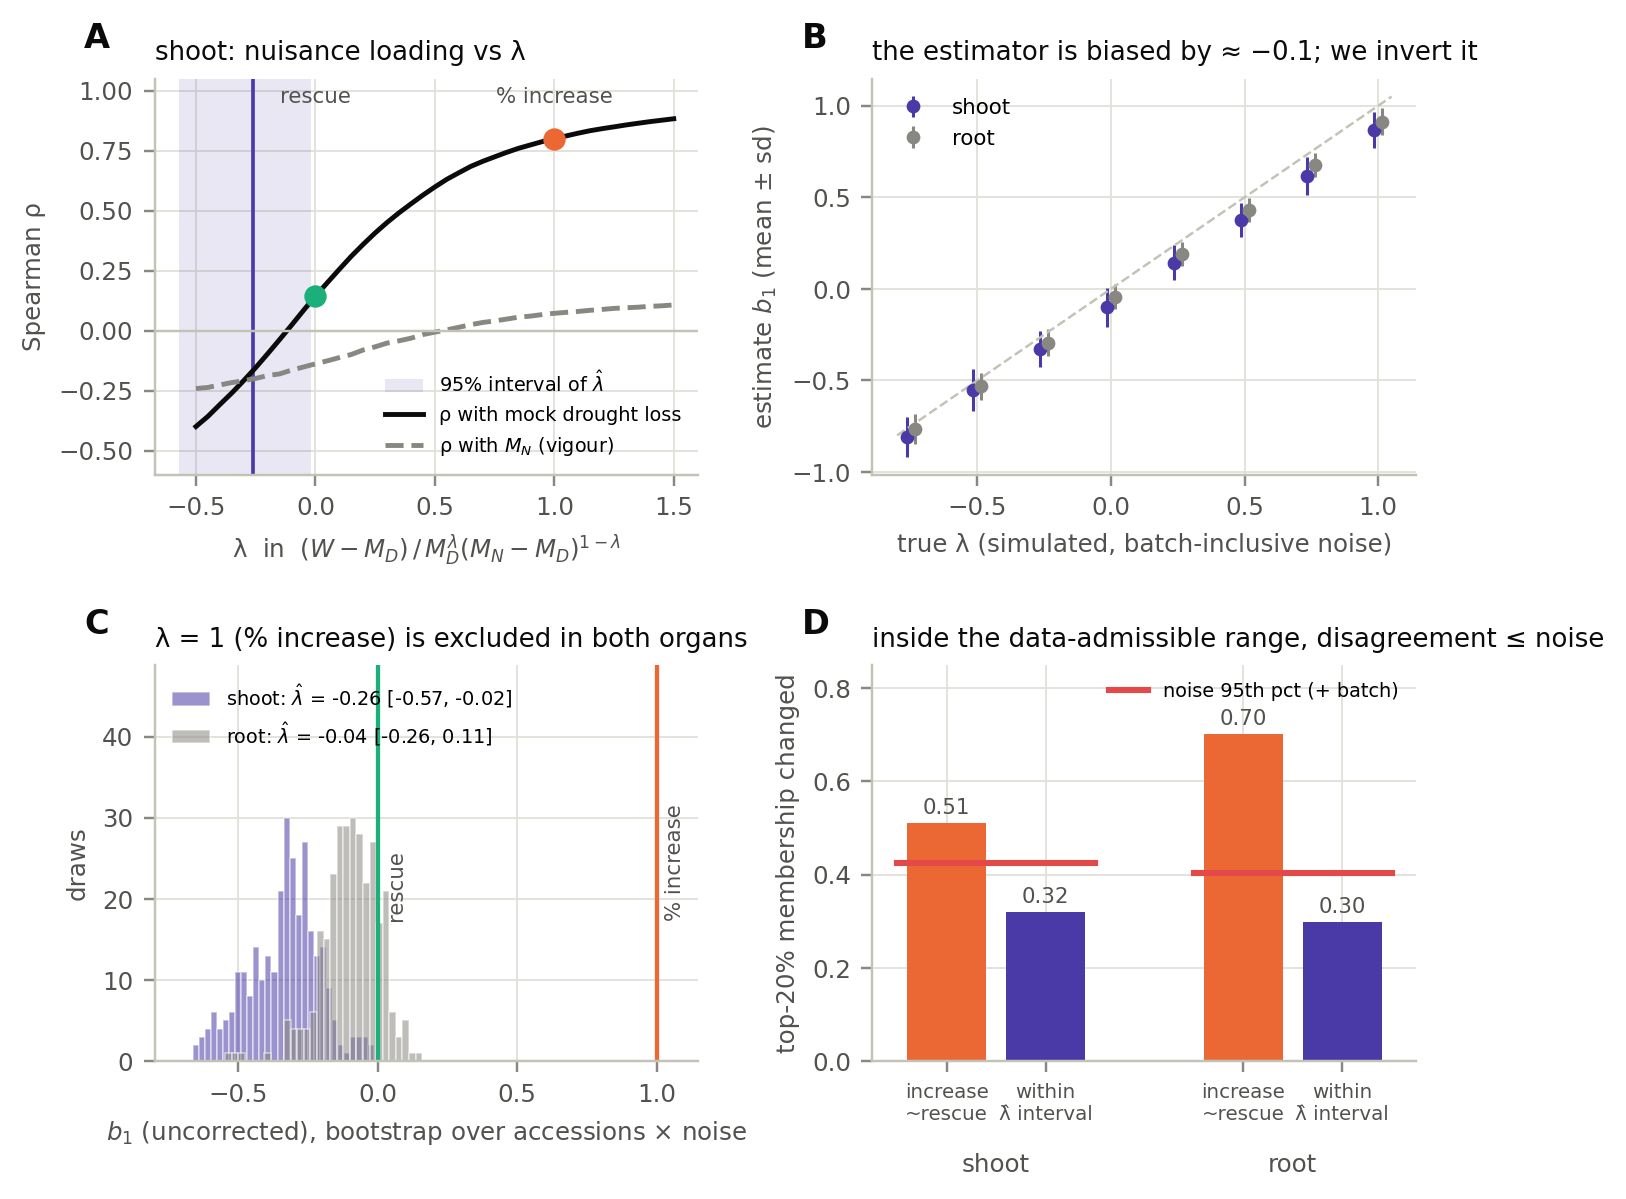
\includegraphics[width=\textwidth]{figures/panel_4_canonical.png}
  \caption{\textbf{The data choose the construction: percentage increase is excluded, and within the admissible range the disagreement falls below noise.}
  (\textbf{A})~Spearman loading of $\flam$ on mock drought loss (solid) and on vigour $\MN$ (dashed) as $\lambda$ varies, shoot. At $\lambda=1$ (percentage increase) the loading on drought loss is 0.80. Near $\lambda=0$ (rescue) both loadings are small. The shaded band is the 95\% interval of the corrected $\lamhat$.
  (\textbf{B})~Recovery of a known $\lambda^*$ from simulated screens with batch-inclusive noise (200 replicates per point). The least-squares slope is biased downward by 0.02--0.13, and more so for larger $\lambda^*$. We invert the curve.
  (\textbf{C})~Bootstrap distribution of the uncorrected slope $b_1$ over accessions and noise. After correction, $\lamhat=-0.26$ [$-0.57$, $-0.02$] (shoot) and $-0.04$ [$-0.26$, $0.11$] (root). $\lambda=1$ lies far outside both.
  (\textbf{D})~Top-20\% change between increase and rescue (orange) compared with change between the two ends of the $\lamhat$ interval (violet), against the batch-inclusive noise ceiling (red). Restricting to data-admissible constructions brings disagreement to 0.32 (shoot) and 0.30 (root), below the ceilings of 0.43 and 0.40.}
  \label{fig:can}
\end{figure*}

\subsection{Letting the data choose}
\label{sec:res-can}

\paragraph{The estimate (\Cref{fig:can}).} The uncorrected fit of
\eqref{eq:loglin} gives $b_1=-0.34$ [$-0.63$, $-0.12$] in shoot and
$-0.09$ [$-0.30$, $0.06$] in root. Simulation shows the estimator is
attenuated by $0.10$ (shoot) and $0.04$ (root) near $\lambda^*=0$.
Correcting gives
\[
  \lamhat_{\mathrm{shoot}}=-0.26\ [-0.57,-0.02],\qquad
  \lamhat_{\mathrm{root}}=-0.04\ [-0.26,\ 0.11].
\]
Percentage increase ($\lambda=1$) is excluded with a wide margin in both
organs. Rescue ($\lambda=0$) lies inside the root interval and just
beyond the upper end of the shoot interval ($-0.02$). We adopt $f_{\lamhat}$, per organ, as
the \emph{canonical} construction. For practical purposes it is rescue:
the two correlate at $\ge0.88$ in tier assignment and never certify
opposite orders.

\paragraph{Scale invariance of the mechanism.} The mechanism
\eqref{eq:gen} predicts $b_1+b_2=1$. The estimate is attenuated too:
under exact invariance, simulation gives $0.81\pm0.17$ (shoot) and
$0.86\pm0.12$ (root).
\begin{itemize}[leftmargin=1.3em,itemsep=1pt]
  \item \emph{Shoot.} The observed $0.61$ is within 1.2 simulation
  standard deviations, so it is compatible with scale invariance.
  \item \emph{Root.} The observed $0.48$ is 3.2 standard deviations below,
  so it is not.
\end{itemize}
Larger root systems gain proportionally less. Correspondingly, no member
of the $\lambda$ family removes the root loading on vigour: at
$\lambda\approx0$, $\rho(\flam,\MN)=-0.34$. In root, the vigour
dependence should be handled in the association model, by entering
$\log\MN$ as a covariate, rather than by the phenotype.

\paragraph{Does canonicalisation restore construction independence?}
Within the data-admissible interval of $\lambda$, the top-20\% change
between the two interval ends is 0.32 (shoot) and 0.30 (root). Both are
below the batch-inclusive noise ceilings of 0.43 and 0.40. The
disagreement between the constructions in use (0.51 and 0.70) exceeds
them. \emph{Once the data are allowed to choose, the residual choice no
longer changes the verdict more than noise does.}

\begin{figure*}[!htbp]
  \centering
  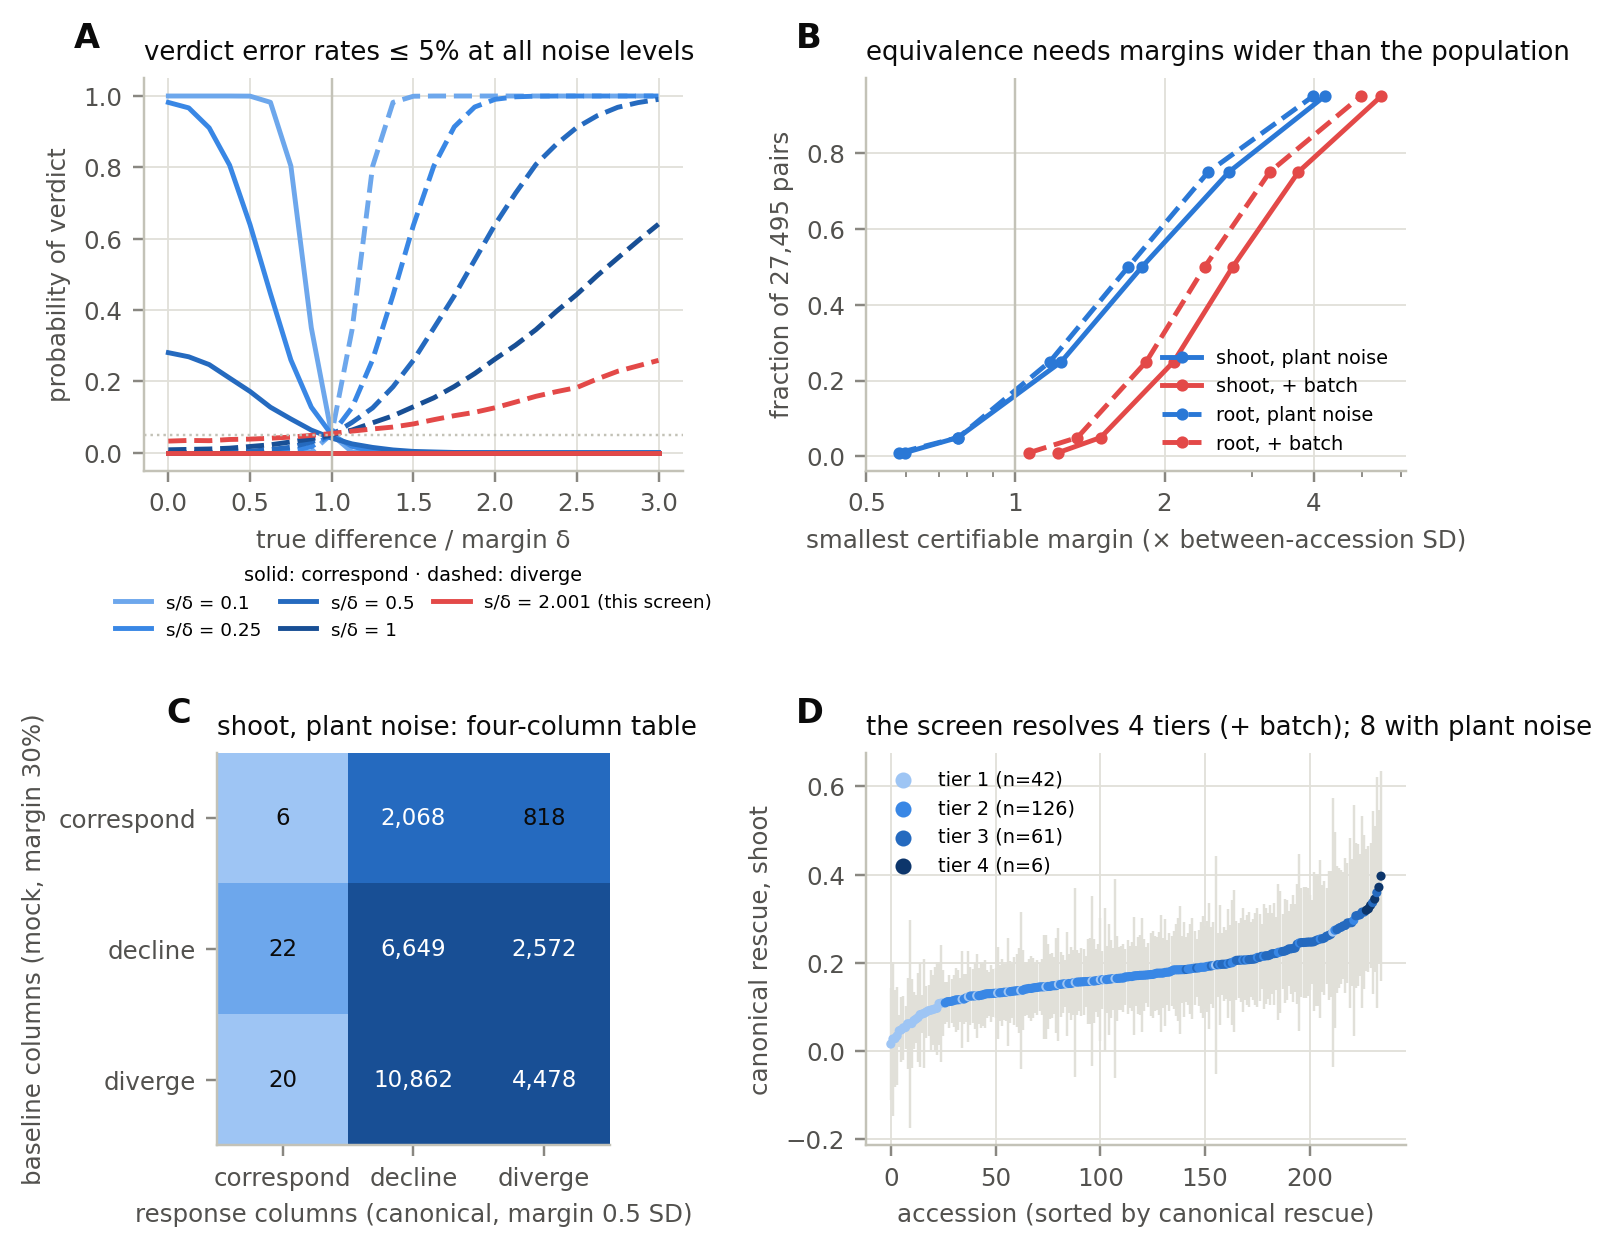
\includegraphics[width=\textwidth]{figures/panel_5_four_column.png}
  \caption{\textbf{The verdict is calibrated, and the screen can certify divergence but almost never equivalence.}
  (\textbf{A})~Operating characteristics of \Cref{def:verdict} by simulation, at five ratios of pair standard error to margin. Solid lines: probability of \CC; dashed lines: probability of \DD. False correspondence beyond the margin never exceeds 0.051 (Monte Carlo error 0.001). False divergence within the margin never exceeds 0.054, which is the bound of \Cref{prop:error}(ii). At this screen's ratio (red, $s/\delta=2$), \CC\ is unreachable.
  (\textbf{B})~Cumulative distribution over all 27,495 pairs of the minimum certifiable margin (\Cref{def:dmin}), in units of the between-accession standard deviation. With plant noise the median pair needs 1.7--1.8 SD; with batch 2.4--2.8 SD. Only 0.07\% (shoot) and 0.55\% (root) of pairs certify below 1 SD under M3.
  (\textbf{C})~The four-column table for shoot under plant noise (baseline margin 30\%, response margin 0.5 SD). There are 818 false friends (\CC, \DD) and 20 convergent pairs (\DD, \CC). Most pairs decline in at least one column.
  (\textbf{D})~Canonical rescue with 95\% intervals, coloured by resolution tier (\Cref{def:depth}). Under M3 the screen resolves four tiers in shoot (42, 126, 61 and 6 accessions); under plant noise it resolves eight.}
  \label{fig:four}
\end{figure*}

\subsection{Four columns and the limits of certification}
\label{sec:res-four}

\paragraph{Calibration (\Cref{fig:four}A).} Across five noise levels,
false correspondence is at most 0.051 and false divergence at most
0.054, as \Cref{prop:error} requires. The verdict does what it claims.

\paragraph{Equivalence is out of reach (\Cref{fig:four}B).} This screen's
ratio of pair standard error to a margin of 0.5 between-accession SD is
2.0. At that ratio \Cref{def:verdict} can almost never return \CC. The
minimum-certifiable-margin distribution makes the limitation exact:
\begin{itemize}[leftmargin=1.3em,itemsep=1pt]
  \item under M3 the median pair certifies as equivalent only at 2.75 SD
  (shoot) or 2.41 SD (root), a margin wider than the spread of the
  population;
  \item even under plant noise alone the medians are 1.80 and 1.69 SD,
  and only 14--16\% of pairs certify below 1 SD.
\end{itemize}
\emph{The screen can say that two accessions differ. It cannot say that
two accessions rescue equally.}

\paragraph{The four-column table (\Cref{fig:four}C).} Under plant noise,
the shoot baseline columns certify 2,892 pairs as equivalent at a 30\%
margin. Of these:
\begin{itemize}[leftmargin=1.3em,itemsep=1pt]
  \item 818 are false friends: certified \emph{different} in response
  despite indistinguishable mock phenotypes. The most extreme include
  IP-Mur-0 with Lu3-30 (canonical rescue 0.05 against 0.31) and Neo-6
  with Uk-1.
  \item 20 pairs are convergent (root: 43).
\end{itemize}
False friends are the informative contrasts for mapping. Their
difference in response cannot be attributed to a difference in baseline
growth or drought sensitivity. Under M3 only 18 shoot false friends
survive, and no convergent pair does, because \CC\ is unreachable in the
response columns.

\paragraph{Resolution depth (\Cref{fig:four}D).} Under M3 the canonical
construction resolves four tiers in shoot and five in root; under plant
noise, eight and ten. Tier assignments of the constructions in use agree
with the canonical tiers only moderately (Spearman 0.44--0.82, lowest for
percentage increase); rescue and the canonical construction agree at
0.88--0.99. The practical reading is that this screen sorts
accessions into a handful of classes, not into 235 ranks.

\subsection{Batch}
\label{sec:res-batch}

Col-0 was sown as an internal control every $\sim$119 rows, which gives
13 usable blocks of 7 plants (\Cref{fig:noise}A). One-way analysis of
variance rejects a common block mean:
\begin{itemize}[leftmargin=1.3em,itemsep=1pt]
  \item shoot: $F=3.76$, $p=1.7\times10^{-4}$;
  \item root: $F=3.12$, $p=1.2\times10^{-3}$.
\end{itemize}
The intraclass correlations \citep{shrout1979} are 0.28 and 0.23. The
between-block standard deviation is 0.43 (shoot) and 0.53 (root) of the
between-accession standard deviation. By method of moments,
$c_b=0.081$ and $0.093$ per cell. The three lines grown twice agree with
this: their two block means differ by 19--42\% (9807: 27.7 against
19.5~mg shoot).

The screen has no block term, so every accession's value carries its
block's offset. Because Col-0 was repeated, the offsets are estimable for
the inoculated--drought cell once block membership is known. The design
already contains the control needed to remove the largest source of
noise it has.

\subsection{Collection site}
\label{sec:res-geo}

Canonical shoot rescue declines towards the east ($\rho=-0.25$ with
longitude, $p=1.2\times10^{-4}$) and weakly towards the north
($\rho=-0.14$, $p=0.037$). Vigour $\MN$ increases in both directions
($\rho=0.15$ and $0.18$). Mock drought loss shows no geographic pattern
in shoot ($p>0.2$).

We ran 20 geographic tests. Two survive Bonferroni correction
($0.05/20=0.0025$): shoot rescue with longitude, and root vigour with
longitude ($\rho=0.20$, $p=0.0024$). Root rescue does not ($p=0.058$). The accessions were not sampled to be
representative, so this is descriptive. A climate covariate from the
collection coordinates \citep{fick2017} is the proper next step; it
would turn the non-random composition of the panel from a reviewer's
objection into a measured variable.

% =====================================================================
\section{Consequences for the screen}
\label{sec:consequences}
% =====================================================================

\begin{figure*}[!htbp]
  \centering
  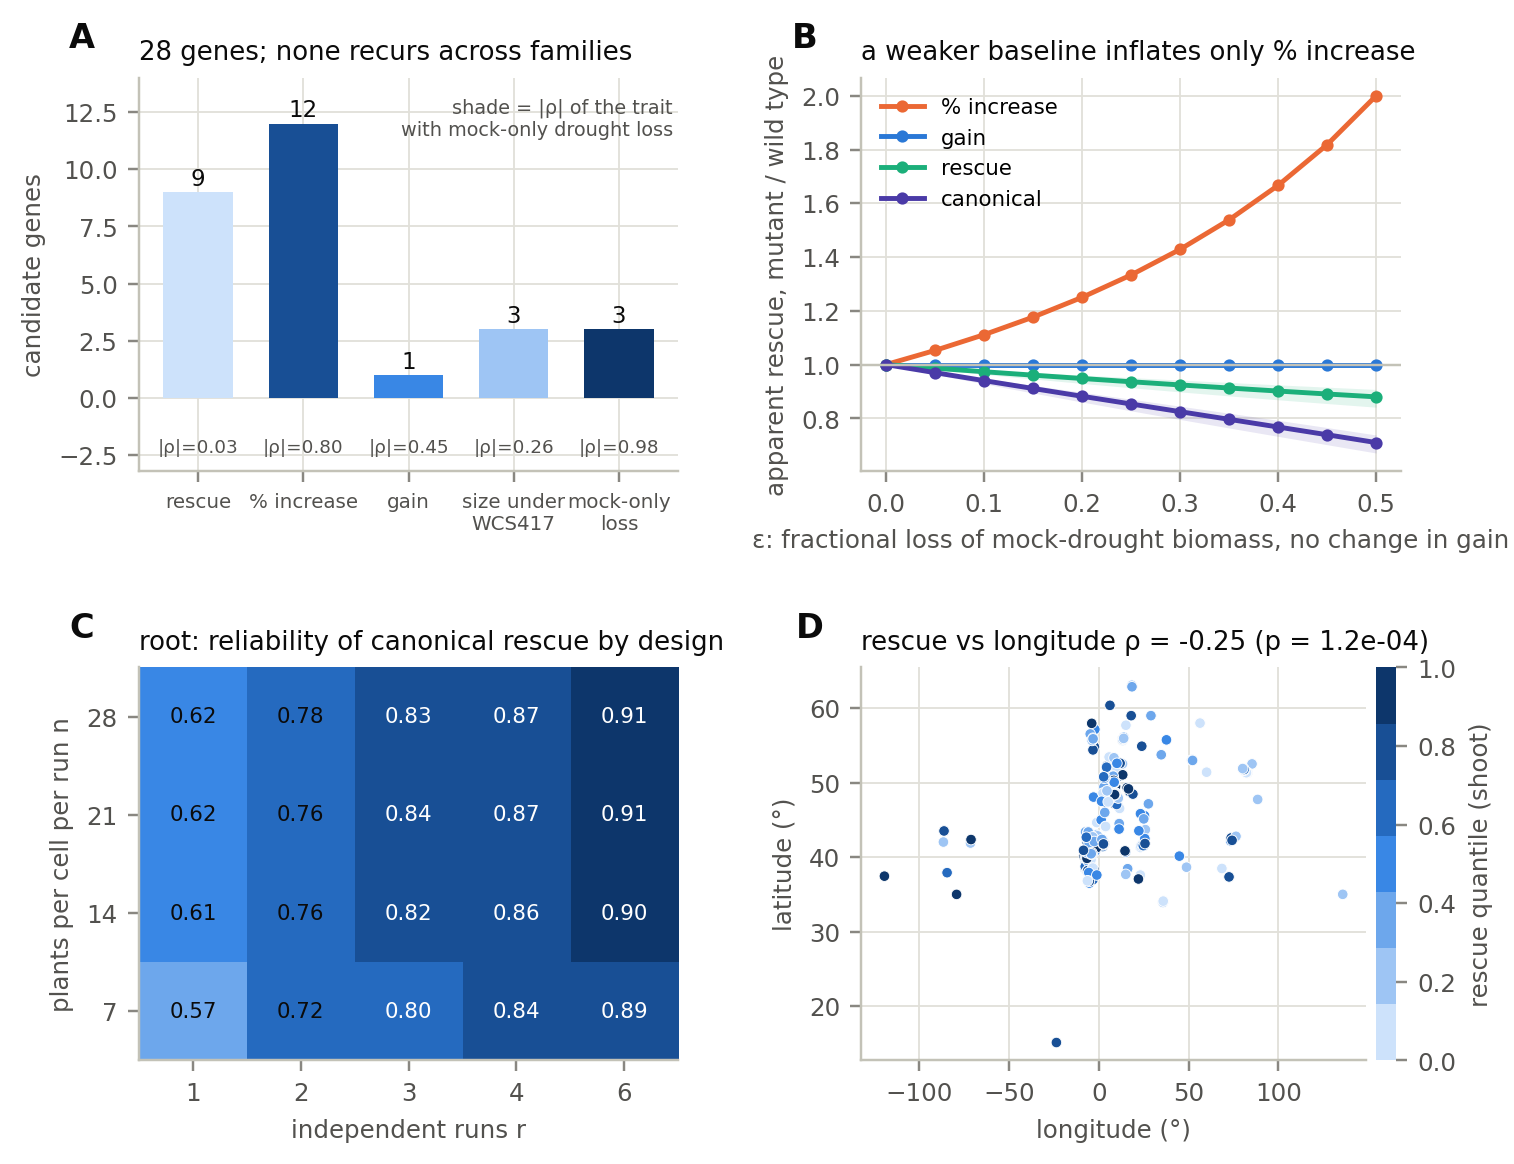
\includegraphics[width=\textwidth]{figures/panel_6_consequences.png}
  \caption{\textbf{Consequences: candidate triage, a check for mutant claims, a replication design, and geography.}
  (\textbf{A})~The 28 candidate genes by the trait family they were found in. Shading is the median $|\rho|$ between that family's traits and mock-only drought loss. No gene recurs across families. Three come from the mock-only family and twelve from percentage increase ($|\rho|=0.80$).
  (\textbf{B})~Apparent change in rescue for a hypothetical mutant whose mock-drought biomass falls by a fraction $\varepsilon$ while its absolute gain and non-stress biomass are unchanged. The median over accessions is shown, with interquartile band. Percentage increase reports up to a two-fold ``enhancement''; gain reports none; rescue and the canonical construction report a decrease.
  (\textbf{C})~Reliability of root canonical rescue by plants per cell $n$ and independent runs $r$.
  (\textbf{D})~Collection sites coloured by the quantile of canonical shoot rescue ($\rho=-0.25$ with longitude).}
  \label{fig:cons}
\end{figure*}

\subsection{Triage of the candidate list}

Of the 40 candidate rows, 28 genes, none appears in more than one trait
family (\Cref{fig:cons}A). The seven genes that appear under several
metrics do so only across near-duplicates of one trait: average and
median of the same trait, or shoot and total, which contains shoot. The
candidates fall into four groups:
\begin{itemize}[leftmargin=1.3em,itemsep=1pt]
  \item \emph{Mock-only (3 genes).} MORN4 (AT1G77660), the antisense
  transcript AT2G07213 and TPS21 (AT5G23960) were found with a trait
  computed without inoculated plants. They are candidates for drought
  sensitivity, not for rescue.
  \item \emph{Percentage increase (12 genes).} These were found with
  traits whose rankings correlate at 0.78--0.81 with drought loss, and
  are at risk of being drought-sensitivity loci.
  \item \emph{Rescue-derived (9 genes).} These are the most interpretable
  candidates for the mutant screen.
  \item \emph{Size and gain (4 genes).} These carry the size loading.
\end{itemize}
This triage says nothing about whether a locus is real. It says which
phenotype it is a locus \emph{for}.

\subsection{Checking mutant claims}

The experimenter reports that mutants in plant iron-uptake genes show
\emph{higher} rescue. That fits a model in which the bacterium supplies
iron independently of the plant \citep{zamioudis2015,verbon2017}.
\Cref{fig:cons}B shows why the claim needs one extra number. Suppose a
mutant only grows worse under drought ($\MD$ reduced by $\varepsilon$)
and receives the same absolute benefit. Then the constructions report:
\begin{itemize}[leftmargin=1.3em,itemsep=1pt]
  \item percentage increase: $1/(1-\varepsilon)$ times more rescue, up to
  $2\times$ at $\varepsilon=0.5$;
  \item gain: no change;
  \item rescue: a decrease, to $0.88\times$ at $\varepsilon=0.5$;
  \item the canonical construction: a larger decrease, to $0.71\times$.
\end{itemize}
The claim of enhanced rescue is established if the absolute gain and the
loss-normalised rescue both rise in the mutants. It is an artefact of the
mutants' weaker baseline if only the percentage increase does.

\subsection{Design}

Batch, not plant number, limits this screen (\Cref{fig:noise}D,
\Cref{fig:cons}C). For shoot canonical rescue, reliability is:
\begin{itemize}[leftmargin=1.3em,itemsep=1pt]
  \item 0.34 at 7 plants in one run (the current design);
  \item 0.36 at 14 plants in one run;
  \item 0.50 at 7 plants in two runs, and 0.61 in three.
\end{itemize}
For root, reliability goes from 0.57 to 0.80 with three runs.
Certifying equivalence at a margin of one true standard deviation becomes
possible (probability 0.49) only for root with 28 plants in six runs, and
it is not reached for shoot on this grid. Three recommendations follow:
\begin{enumerate}[label=(\roman*),leftmargin=1.8em,itemsep=1pt]
  \item Repeat the screen in independent runs rather than adding plants.
  \item Grow the mock and inoculated plants of an accession together, so
  that batch cancels in the gain.
  \item Keep a common control in every block and enter block as a term.
\end{enumerate}

\subsection{The analysis the data now support}

Before any further association scan:
\begin{enumerate}[label=(\arabic*),leftmargin=1.8em,itemsep=1pt]
  \item fix the phenotype to the canonical construction per organ,
  estimated as in \S\ref{sec:methods-lambda};
  \item fit a single model on per-plant data from all cells, with the
  inoculation $\times$ drought interaction as the phenotype and block as
  a term;
  \item enter kinship \citep{yu2006,kang2010} and, for root, $\log\MN$ as
  covariates;
  \item report the resolution depth and the fraction of declined pairs
  alongside any ranking.
\end{enumerate}
The first step needs no new data. The second needs the per-plant mock
and non-stress data, which exist in the laboratory but not in the
workbook.

% =====================================================================
\section{Discussion}
\label{sec:discussion}
% =====================================================================

\paragraph{Rescue as a relation.} The opening observation is simple.
What an accession ``does'' with WCS417 under drought is not a property
the accession carries. It is a relation among four cells, only one of
which is directly the inoculated plant. A number assigned to the
accession is a reading of that relation. Several readings are admissible
and they disagree, and the disagreement is not noise
(\S\ref{sec:res-dep}). This is the familiar statement that
gene-by-environment interaction is the phenotype
\citep{elsoda2014,desmarais2013}, made operational. The object to be
mapped is fixed only when a reading is fixed, and the reading should be
fixed by the data.

\paragraph{Choice of reading as a testable hypothesis.} The $\lambda$
family turns ``which formula?'' into ``which mechanism?''
(\Cref{prop:mechanism}): a multiplicative benefit on stressed biomass, or
a restored fraction of the loss. The data answer that the benefit scales
with the loss and not with the stressed biomass. That is a small
biological result in its own right: WCS417 behaves as if it restores a
share of what drought removes. It also has a methodological consequence.
The trait that yielded twelve of the 28 candidates is the reading the
data reject.

\paragraph{Comparison through four columns.} Comparing accessions by
their response alone treats two different things as one: a difference in
what the bacterium does, and a difference in the plant it does it to.
Carrying the mock baseline as two further columns separates them. The
separation matters most where it is least visible, in false friends.
These are pairs indistinguishable without the bacterium and different
with it, and they are the contrasts a follow-up experiment should use.

\paragraph{Declining to decide.} The third verdict value does work that
no score can. On this screen most pairs \emph{decline}
(\Cref{fig:four}C), and \emph{correspond} is almost unreachable
(\Cref{fig:four}B). A method obliged to return a similarity for every
pair would have returned 27,495 numbers, and nothing in them would have
said that most of those numbers could not support a decision. We regard
the minimum certifiable margin as the single most useful summary of a
screen of this kind. It says how fine a distinction the experiment can
support before any locus is sought.

\paragraph{The absence of loss of rescue.} The screen could have
detected complete loss in most backgrounds, and did not see it. That is
consistent with the experimenter's redundancy hypothesis, in which rescue
runs through several routes and removing one leaves the others. It is
also consistent with the iron result: uptake mutants are rescued more,
not less. Under redundancy, the informative next experiment is
combinatorial. In a network built from the time-resolved transcriptome,
one would ask for the smallest set of genes whose joint removal
disconnects the bacterial signal from the growth outcome, and test that
set as a higher-order mutant. We have not done this; it requires the
transcriptome.

% =====================================================================
\section{Limitations}
\label{sec:limits}
% =====================================================================

\begin{enumerate}[label=\textbf{L\arabic*.},leftmargin=2.1em,itemsep=2pt]
  \item \textbf{Three cells have modelled, not measured, noise.} The
  mock and non-stress spreads are assumed equal in relative terms to the
  inoculated--drought spread (\Cref{ass:noise}). M4 (mock noise
  $\times1.5$) changes no qualitative conclusion, but per-plant data for
  those cells would replace the assumption with a measurement.
  \item \textbf{Batch is estimated from one cell and one genotype.} Col-0
  blocks exist only for inoculated--drought. We assumed the same batch
  coefficient of variation elsewhere and independent batch effects
  across cells; shared trays would make M3 pessimistic.
  \item \textbf{No genotypes.} We did not rerun the association, correct
  it for kinship or population structure, or test any candidate.
  \item \textbf{One run.} Every conclusion about construction
  dependence could be sharpened, or reversed in shoot, by a second run.
  The design analysis shows that a second run is the most valuable single
  addition.
  \item \textbf{The $\lambda$ model is a model.} \eqref{eq:gen} is one
  family of mechanisms. The root rejection of $b_1+b_2=1$ shows that it
  is incomplete there. The simulation-based bias correction assumes the
  noise model.
  \item \textbf{Margins are choices.} The verdicts depend on $\delta$. We
  report sweeps and the minimum certifiable margin, which do not depend
  on a choice, but the four-column table does.
  \item \textbf{$\WN$ is unidentified.} Constructions that use the
  inoculated non-stress plants, for example a full interaction contrast,
  cannot be evaluated from the workbook.
\end{enumerate}

% =====================================================================
\section{Conclusion}
\label{sec:conclusion}
% =====================================================================

A screen for rhizobacterial drought rescue measures a relation, and its
derived traits are readings of that relation. On 235 \emph{Arabidopsis}
accessions inoculated with WCS417, the readings in use disagree beyond
noise in root, and under plant-level noise they certify hundreds of pairs
in opposite order. Percentage increase, the source of the largest group
of candidate loci, is the reading the data reject, because it largely
ranks drought sensitivity. The data select a loss-normalised rescue.
Within the admissible range the choice stops mattering more than noise.
Compared through four columns with a calibrated three-valued verdict, the
screen certifies divergence but almost never equivalence, and resolves
four to five tiers of rescue. Its largest source of noise is batch, which
its own Col-0 control can measure and remove. The next steps are the
phenotype fixed before mapping, the per-plant model with block and
kinship, a second independent run, and a retest of Per-1. None requires
a new idea, only the decision to let the data choose the phenotype and
the discipline to report when they cannot decide.

\subsection*{Data and code availability}
The screen's data are unpublished and belong to the laboratory that
generated them. The validation suite (\texttt{validation/}) regenerates
every number in this paper from the workbook, deterministically, from
seed 417, in about ten seconds. Results are written to \texttt{results/}
as one JSON file per experiment (E1--E12), and figures are rebuilt from
those files by \texttt{validation/make\_figures.py}. Analyses use NumPy,
SciPy, pandas, scikit-learn and Matplotlib
\citep{harris2020,virtanen2020,mckinney2010,pedregosa2011,hunter2007};
the accompanying interactive specification uses D3 \citep{bostock2011}.

\subsection*{Acknowledgements}
We thank the laboratory that designed and ran the screen, generated all
data analysed here, and described the experiment in detail.

\subsection*{Conflicts of interest}
None declared.

\bibliography{references}

\end{document}
